\chapter{Resultados}

Tras haber definido la solución y acoplado los datos conforme a esta, el algoritmo está listo para ser probado y comenzar con la fase de experimentación que se describe en el Capítulo actual.

\section{Parametrización}

Luego de la ejecución de \textit{i-race}, cuyo tiempo de ejecución fue aproximadamente de 75 horas, los resultados (mostrados en la tabla \ref{tab:5.1}) indican los mejores parámetros a utilizar en el algoritmo \textit{SA}, de los cuales, tras observar la cantidad de ciclos totales requeridos para cada caso, se escogen los fila con ID 9 al encontrarse en el primer lugar de la tabla. Con esto en mente, si se desea reducir el tiempo de ejecución, se recomienda escoger los parámetros con ID 2 en la segunda fila, pues sólo agrega 42 segundos al intervalo máximo a cambio de 150 iteraciones internas menos.

\begin{table}[H]
\centering
\def\arraystretch{1.8}
\captionsetup{justification=centering}
\caption{Resultados de i-race}
\label{tab:5.1}
\begin{tabular}{|c|c|c|c|c|}
\hline
\textbf{ID} & \textbf{Iteraciones internas} & \textbf{Temperatura} & \textbf{Alfa} & \textbf{Intervalo máximo} \\
\hline
9 & 250 & 20583 & 0.56 & 132         \\ \hline
2 & 100 & 4927 & 0.51 & 174          \\ \hline
22 & 100 & 791 & 0.53 & 144          \\ \hline
8 & 250 & 11360 & 0.58 & 152         \\ \hline
\end{tabular}
\caption*{\textbf{Fuente}: Elaboración Propia, 2021}
\end{table}

\section{Tiempos de ejecución}

Sólo a modo de documentación, pues existen una serie de elementos incontrolables que pueden afectarlo, es que se calcula el tiempo de ejecución de cada una de las ejecuciones del algoritmo. Los resultados de 15 ejecuciones entregaron un promedio de 26,52 minutos con un máximo de 33.34 minutos y un mínimo de 17.53.

\section{Evaluación}

A continuación se detallan los resultados de los experimentos propuestos en la sección 3.2.2, además de un análisis sobre cada uno de estos.

\subsection{Convergencia del algoritmo}

Tras ejecutar el algoritmo 3 veces para 1 \textit{Marine} se obtienen, además de los órdenes de construcción, los gráficos que muestran como el puntaje de las generaciones de cada iteración oscila al tratarse de \textit{Simulated Annealing}, pues este algoritmo tiene una probabilidad de escoger una solución peor (con un puntaje más alto), pero que siempre escoge una solución con un mejor puntaje. Esta oscilación se detiene conforme avanzan las iteraciones, pues la probabilidad de aceptación es cada vez menor. Los gráficos muestran en una tonalidad celeste esta oscilación al indicar el puntaje $P_{SA}$ de $G_{SA}$ en el tiempo, mientras que en azul se observa la mejor solución $P_{Best}$ encontrada de todas las generaciones en el tiempo.

A continuación se muestran los gráficos resultantes en cada ejecución del algoritmo:
%de momento solo los 3 primeros%

\begin{figure}[H]
	\centering
	\captionsetup{justification=centering}
	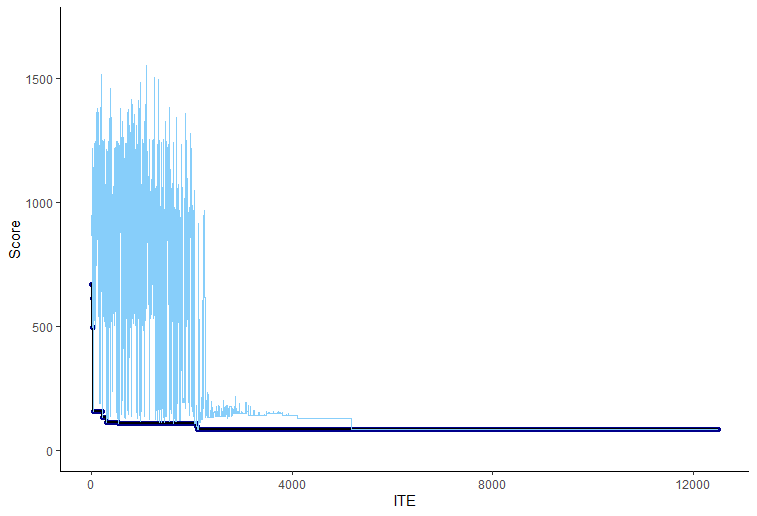
\includegraphics[scale=0.65]{images/marine1.png}
	\captionimg{Gráfico de generaciones de SA del Experimento 1: primera ejecución para 1 Marine}{Elaboración propia, 2021}
	\label{fig:10}
\end{figure}

\begin{figure}[H]
	\centering
	\captionsetup{justification=centering}
	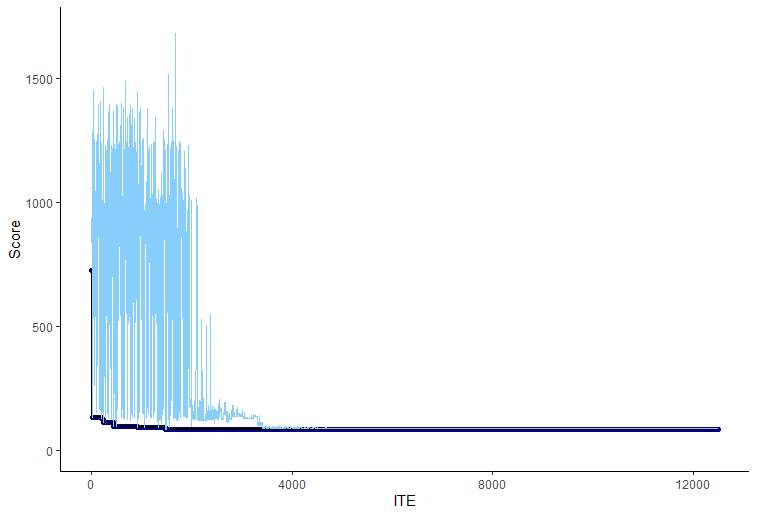
\includegraphics[scale=0.65]{images/marine2.png}
	\captionimg{Gráfico de generaciones de SA del Experimento 1: segunda ejecución para 1 Marine}{Elaboración propia, 2021}
	\label{fig:11}
\end{figure}

\begin{figure}[H]
	\centering
	\captionsetup{justification=centering}
	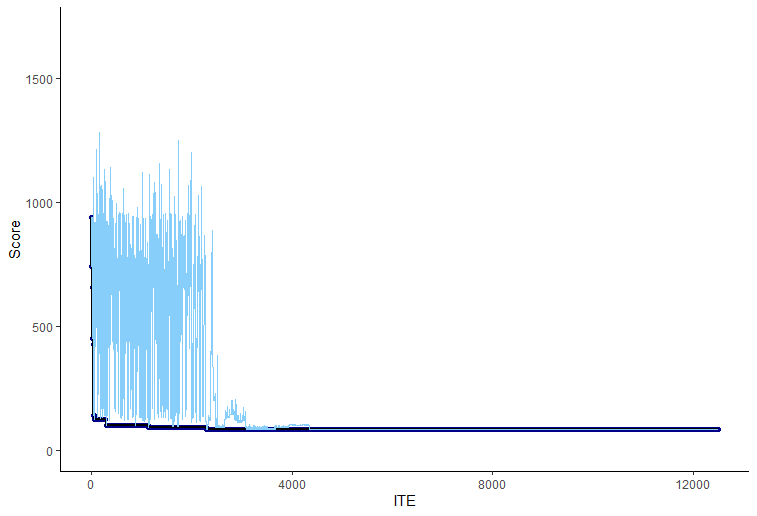
\includegraphics[scale=0.65]{images/marine3.png}
	\captionimg{Gráfico de generaciones de SA del Experimento 1: tercera ejecución para 1 Marine}{Elaboración propia, 2021}
	\label{fig:12}
\end{figure}

Si bien el algoritmo posee un alto grado de aleatoriedad y las generaciones para una misma entidad son similares entre ellas, pues se puede ver como SA deja su oscilación característica alrededor del mismo punto alrededor de las 4000 iteraciones. También es común entre las soluciones el hecho de que la mejor solución rápidamente se reduce en las primeras iteraciones, mejorando lentamente a partir de aquí hasta que alcanza el equilibrio con un puntaje de 84.

\begin{table}[H]
\centering
\def\arraystretch{1.2}
\captionsetup{justification=centering}
\caption{Resultados de SA: primera ejecución para 1 Marine}
\label{tab:marine1}
\begin{tabular}{|c|c|}
\hline
\textbf{Tiempo (en minutos)} & \textbf{Acción} \\
\hline
0:08	&  Supply Depot	 \\ 
0:16	&  SCV	  \\
0:37	&  Barracks	  \\
0:45	&  SCV	  \\
1:01	&  Refinery	  \\
1:07	&  SCV	  \\
1:14	&  Refinery	  \\
1:23	&  Marine \\ \hline
\end{tabular}
\caption*{\textbf{Fuente}: Elaboración Propia, 2021}
\end{table}

\begin{table}[H]
\centering
\def\arraystretch{1.2}
\captionsetup{justification=centering}
\caption{Resultados de SA: segunda ejecución para 1 Marine}
\label{tab:marine2}
\begin{tabular}{|c|c|}
\hline
\textbf{Tiempo (en minutos)} & \textbf{Acción} \\
\hline
0:07	&  Supply Depot	 \\ 
0:15	&  SCV	  \\
0:37	&  Barracks	  \\
0:49	&  SCV	  \\
0:56	&  Refinery	  \\
1:10	&  Refinery	  \\
1:18	&  SCV	  \\
1:23	&  Marine \\ \hline
\end{tabular}
\caption*{\textbf{Fuente}: Elaboración Propia, 2021}
\end{table}

\begin{table}[H]
\centering
\def\arraystretch{1.2}
\captionsetup{justification=centering}
\caption{Resultados de SA: tercera ejecución para 1 Marine}
\label{tab:marine3}
\begin{tabular}{|c|c|}
\hline
\textbf{Tiempo (en minutos)} & \textbf{Acción} \\
\hline
0:08	&  Supply Depot	 \\ 
0:15	&  SCV	  \\
0:37	&  Barracks	  \\
0:49	&  SCV	  \\
1:04	&  SCV  \\
1:09	&  Refinery	  \\
1:18	&  Refinery	  \\
1:23	&  Marine \\ \hline
\end{tabular}
\caption*{\textbf{Fuente}: Elaboración Propia, 2021}
\end{table}

Aquí se observa que en las 3 ejecuciones, tanto la cantidad de unidades como el tiempo total son los mismos, pues todos tienen 1 \textit{Supply Depot}, 3 \textit{SCV}, 2 \textit{Refineries} y 1 \textit{Barracks} antes de alcanzar al Marine en el minuto 1:23. Es interesante observar como el algoritmo parece optimizar el camino a la entidad especificada, pues para construir un \textit{Marine} se requiere del edificio \textit{Barracks}, el cual comienza su creación en las 3 ocasiones con la misma marca de tiempo de 0:37 minutos para luego, exactamente 46 segundos después cuando es creado y se vuelve utilizable en el juego, crear un Marine al minuto 1:23. Por otro lado, aquellas entidades que no afectan directamente a la creación del Marine tienen distintas marcas de tiempo y tienen un orden distinto en las 3 ocasiones.

\subsection{Órdenes de construcción de profesionales}

Como se indica en la sección 3.2.2.2, se compararon órdenes de construcción obtenidos con algunos órdenes de construcción de profesionales en torneos oficiales, recopilados por la comunidad de StarCraft II. A continuación se pueden observar las tablas que contrastan los órdenes de construcción entregados por SA con los órdenes de construcción de profesionales, los cuales no muestran las construcciones de trabajadores para acortar el largo de las tablas.

\begin{table}[H]
\centering
\def\arraystretch{1.2}
\captionsetup{justification=centering}
\caption{Orden de construcción de ByuN para 1 Marine}
\label{tab:marineByun}
\begin{tabular}{|c|c|}
\hline
\textbf{Tiempo (en minutos)} & \textbf{Acción} \\
\hline
0:17 &	  Supply Depot	  \\
0:39 &	  Barracks	  \\
0:42 &	  Refinery	  \\
1:25 &	  Marine \\ \hline
\end{tabular}
\caption*{\textbf{Fuente}: Spawning Tool, 2021}
\end{table}

Si se confronta la tabla \ref{tab:marine3} con el orden de construcción encontrado más rápido para llegar a un \textit{Marine}, se observa que tanto la cantidad de entidades como el tiempo es mejor en el orden de construcción obtenido por el algoritmo, pues acorta 2 segundos de la solución que propone el jugador y crea un \textit{Refinery} extra que ayuda a mejorar la cantidad de gas vespeno a recolectar.

\begin{table}[H]
\centering
\def\arraystretch{1.2}
\captionsetup{justification=centering}
\caption{Resultados de SA para 1 Starport}
\label{tab:5.4}
\begin{tabular}{|c|c|}
\hline
\textbf{Tiempo (en minutos)} & \textbf{Acción} \\
\hline
0:14 & Refinery \\ 
0:30 & Refinery \\ 
0:48 & Supply Depot \\ 
1:15 & Barracks \\ 
2:01 & Marine \\ 
2:21 & Factory \\
2:33 & Marine \\
2:54 & Reaper \\ 
3:08 & Starport \\ \hline
\end{tabular}
\caption*{\textbf{Fuente}: Elaboración Propia, 2021}
\end{table}

\begin{table}[H]
\centering
\def\arraystretch{1.2}
\captionsetup{justification=centering}
\caption{DreamHack SC2 Masters 2021 Summer: orden de construcción de 1 Starport por LiquidClem}
\label{tab:5.5}
\begin{tabular}{|c|c|}
\hline
\textbf{Tiempo (en minutos)} & \textbf{Acción} \\
\hline
0:16 &	  Supply Depot	  \\
0:39 &	  Barracks	  \\
0:43 &	  Refinery	  \\
1:27 &	  Reaper, Orbital Command	  \\
1:39 &	  Command Center	  \\
1:47 &	  Supply Depot	  \\
1:58 &	  Marine	  \\
2:11 &	  Factory	  \\
2:21 &	  Reactor (Barracks)	\\  
2:39 &	  Command Center	\\  
2:52 &	  Orbital Command	\\  
2:58 &	  Starport	  \\ \hline
\end{tabular}
\caption*{\textbf{Fuente}: Spawning Tool, 2021}
\end{table}

La tabla \ref{tab:5.4} muestra el orden de construcción obtenido de SA mientras que la tabla \ref{tab:5.5} muestra el orden de construcción con el cual se comparan los resultados del algoritmo. En esta ocasión el orden de construcción de SA presenta una diferencia de 10 segundos en contra para llegar al \textit{Starport}, además de que se obtienen menos entidades que en el orden de construcción de un jugador en un torneo oficial. Con esto en mente, el orden de construcción de SA tiene un \textit{Marine} extra, lo cual le deja en ventaja si sólo se observan las unidades totales.

\begin{table}[H]
\centering
\def\arraystretch{1.2}
\captionsetup{justification=centering}
\caption{Resultados del Experimento 2: SA para 2 Hellions}
\label{tab:5.9}
\begin{tabular}{|c|c|}
\hline
\textbf{Tiempo (en minutos)} & \textbf{Acción} \\
\hline
0:14 & Supply Depot\\ 
0:34 & Refinery \\ 
0:58 & Refinery \\ 
1:31 & Barracks \\ 
2:03 & Supply Depot \\
2:17 & Reaper \\
2:34 & Factory \\
2:50 & Reaper \\ 
3:05 & Bunker \\ 
3:17 & Hellion \\
3:25 & Marine \\
3:38 & Hellion \\\hline
\end{tabular}
\caption*{\textbf{Fuente}: Elaboración Propia, 2021}
\end{table}

\begin{table}[H]
\centering
\def\arraystretch{1.2}
\captionsetup{justification=centering}
\caption{DreamHack SC2 Masters 2021 Summer: orden de construcción de 2 Hellions por LiquidClem}
\label{tab:5.11}
\begin{tabular}{|c|c|}
\hline
\textbf{Tiempo (en minutos)} & \textbf{Acción} \\
\hline
0:16 &	  Supply Depot	  \\
0:39 &	  Barracks	  \\
0:43 &	  Refinery	  \\
1:27 &	  Reaper, Orbital Command	  \\
1:39 &	  Command Center	  \\
1:47 &	  Supply Depot	  \\
1:58 &	  Marine	  \\
2:11 &	  Factory	  \\
2:21 &	  Reactor (Barracks)	\\  
2:39 &	  Command Center	\\  
2:52 &	  Orbital Command	\\  
2:58 &	  Starport	  \\
3:03 &	  Refinery	  \\
3:11 &	  Hellion \\
3:32 &	  Hellion \\ \hline
\end{tabular}
\caption*{\textbf{Fuente}: Spawning Tool, 2021}
\end{table}

En este caso se tiene una solución algo más compleja debido a los requisitos totales de un Hellion, lo que queda en evidencia al observar que la solución en la tabla \ref{tab:5.11} se acerca a la de LiquidClem, pero no consigue mejorar el tiempo de este, pues es 6 segundos más rápida que la obtenida con el algoritmo SA. En este caso, aunque la cantidad de entidades es, también, mayor en el orden de construcción del profesional, se puede observar como la cantidad de unidades es mejor en la solución de SA, pues incluye un \textit{Reaper} extra.

\begin{table}[H]
\centering
\def\arraystretch{1.2}
\captionsetup{justification=centering}
\caption{Resultados del Experimento 2: SA para 4 Siege Tanks}
\label{tab:5.3}
\begin{tabular}{|c|c|}
\hline
\textbf{Tiempo (en minutos)} & \textbf{Acción} \\
\hline
0:14 & Supply Depot \\ 
0:34 & Refinery \\ 
0:54 & Refinery \\ 
1:10 & Barracks \\ 
1:54 & Supply Depot \\ 
2:14 & Marine \\
2:32 & Bunker \\
2:40 & Marine \\ 
3:00 & Marine \\ 
3:11 & Factory \\ 
3:22 & Reactor (Barracks) \\ 
3:47 & Supply Depot \\ 
3:54 & Tech Lab (Factory) \\ 
4:02 & Marine \\ 
4:06 & Reaper \\ 
4:22 & Siege Tank \\ 
4:38 & Siege Tank \\ 
4:46 & Marine \\ 
5:01 & Supply Depot \\ 
5:14 & Reaper \\ 
5:28 & Siege Tank \\ 
5:50 & Siege Tank \\ \hline
\end{tabular}
\caption*{\textbf{Fuente}: Elaboración Propia, 2021}
\end{table}

\begin{table}[H]
\centering
\def\arraystretch{1.2}
\captionsetup{justification=centering}
\caption{Fragmento (desde minuto 3:30) del orden de construcción de Pfoe para 4 Siege Tanks}
\label{tab:5.6}
\begin{tabular}{|c|c|}
\hline
\textbf{Tiempo (en minutos)} & \textbf{Acción} \\
\hline
3:30	&  Medivac	 \\ 
3:33	&  Marine x2, Supply Depot	  \\
3:43	&  Refinery	  \\
3:46	&  Tech Lab (Factory)	  \\
3:51	&  Marine x2	  \\
4:00	&  Tech Lab (Starport)	  \\
4:07	&  Siege Tank	  \\
4:11	&  Supply Depot	  \\
4:17	&  Barracks x2	  \\
4:23	&  Raven	  \\
4:31	&  Engineering Bay	  \\
4:40	&  Siege Tank	  \\
4:42	&  Refinery	  \\
4:48	&  Marine	  \\
4:57	&  Terran Infantry Weapons Level 1	  \\
5:04	&  Tech Lab (Barracks)	\\  
5:13	&  Stimpack	  \\
5:19	&  Siege Tank	  \\
5:23	&  Reactor (Starport)	  \\
5:30	&  Combat Shield	  \\
5:48	&  Marauder x2	  \\
5:52	&  Siege Tank \\ \hline
\end{tabular}
\caption*{\textbf{Fuente}: Elaboración Propia, 2021}
\end{table}

En este objetivo, el tiempo es menor en el orden de construcción del algoritmo SA por 2 segundos, pero el orden de construcción de Pfoe entrega una mayor cantidad y diversidad de entidades, consiguiendo incluso tecnologías que mejoran algunas unidades creadas en la misma secuencia.

Con las comparaciones anteriores queda en evidencia que el algoritmo está a la par con los órdenes de construcción usados por profesionales y jugadores de alto rango, consiguiendo incluso acortar algunos segundos para algunas de estas soluciones y, en algunos casos, obtener un mejor ejército si lo único que se busca es atacar al oponente.

\subsection{Aplicación dentro del juego}

Tras probar en el videojuego los órdenes de construcción descritos en las secciones anteriores, se deduce que si es posible llevarlos a cabo, aunque se requiere de un buen manejo de los controles de StarCraft II, pues no es sencillo, sin antes practicar o realizar repetidos intentos, seguir las secuencias teniendo menos de un segundo para realizar la acción en el tiempo específico.

A continuación se muestran capturas de pantalla del juego con los órdenes de construcción resultantes para 1 \textit{Marine} (tabla \ref{tab:marine3}) y 2 \textit{Hellions} (tabla \ref{tab:5.11}), los cuales se acercan lo más posible a los órdenes de construcción, pues igualarlos a la perfección puede resultar en varias horas de intentos, aunque queda en evidencia que los tiempos se cumplen y son posibles en el juego.

\begin{figure}[H]
	\centering
	\captionsetup{justification=centering}
	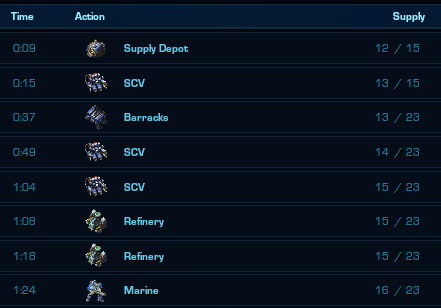
\includegraphics[keepaspectratio]{images/boMarine.png}
	\captionimg{Orden de construcción para un Marine dentro del juego}{Elaboración propia, 2021}
	\label{fig:marineIG}
\end{figure}

\begin{figure}[H]
	\centering
	\captionsetup{justification=centering}
	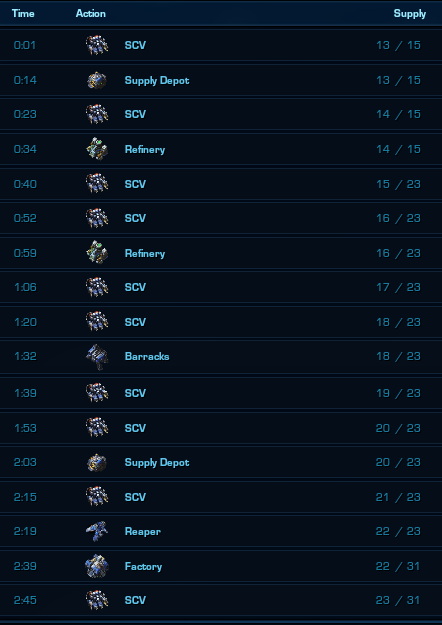
\includegraphics[keepaspectratio]{images/boHellion.png}
	\captionimg{Parte de un orden de construcción para dos Hellion dentro del juego}{Elaboración propia, 2021}
	\label{fig:marineIG}
\end{figure}